\begin{mdframed}[style=warning]
	\begin{ejercicio}
		\textbf{Conceptos.}
		\begin{enumerate}
			\item Una fuerza conservariva mueve a una partícula de $A$ a $B$. ¿A través de qué trayectoria realiza más trabajo sobre la partícula? Responda lo mismo para el caso de una fuerza no conservativa. Explique su respuesta.
			\begin{center}
				


\tikzset{every picture/.style={line width=0.75pt}} %set default line width to 0.75pt        

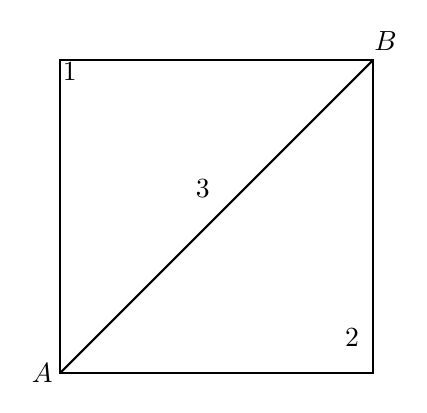
\begin{tikzpicture}[x=0.75pt,y=0.75pt,yscale=-1,xscale=1]
%uncomment if require: \path (0,300); %set diagram left start at 0, and has height of 300

%Shape: Square [id:dp04181596515073305] 
\draw   (232,54) -- (383,54) -- (383,205) -- (232,205) -- cycle ;
%Straight Lines [id:da10667103567095948] 
\draw    (383,54) -- (232,205) ;

% Text Node
\draw (232,54) node [anchor=north west][inner sep=0.75pt]    {$1$};
% Text Node
\draw (368,182) node [anchor=north west][inner sep=0.75pt]    {$2$};
% Text Node
\draw (296,110) node [anchor=north west][inner sep=0.75pt]    {$3$};
% Text Node
\draw (217,199) node [anchor=north west][inner sep=0.75pt]    {$A$};
% Text Node
\draw (382,39) node [anchor=north west][inner sep=0.75pt]    {$B$};


\end{tikzpicture}

			\end{center}
		\end{enumerate}
	\end{ejercicio}
\end{mdframed}











\begin{mdframed}[style=warning]
	\begin{ejercicio}
		Una partícula se puede deslizar a lo largo de una pista con extremos elevados y una parte central plana. La parte plana tiene longitud $L$ con coeficiente de fricción $\mu$, mientras que los extremos tienen altura $h = L/2$ y son lisos. A qué distancia del extremo izquierdo de la parte plana se detiene la partícula?
	\end{ejercicio}
\end{mdframed}












\begin{mdframed}[style=warning]
	\begin{ejercicio}
		Un bloque de masa $m$ se desliza sin roce por una rampa cuya forma está definida por la ecuación:
			$$ \qty[\frac{x - a}{a}]^2 + \qty[\frac{y - b}{b}]^2 = 1. $$
		La partícula parte desde el reposo en el punto $A$ y al alcanzar el punto $B$ sigue deslizando sobre una superficie horizontal rugosa de largo $d$ para finalmente chocar con la plataforma de masa despreciable que está fija a dos resortes, como se indica en la figura. Como resultado del impacto, la partícula se detiene cuando los resortes se comprimen una distancia $\Delta x$. Considerando que la constante elástica de ambos resortes es $k$, calcule el coeficiente de roce cinético $\mu$ que debe existir entre la partícula y la superficie horizontal.
		\begin{figure}[H]
			\centering
			\includegraphics[scale=0.5]{./img/p1.png}
			\caption{Ejercicio 3.}
		\end{figure}
	\end{ejercicio}
	\noindent \textit{Hint: Reduzca los resortes en paralelo a un único resorte equivalente.}
\end{mdframed}










\begin{mdframed}[style=warning]
	\begin{ejercicio}
		El clavo $\mathcal{O}'$ está situado a una distancia $d$ por debajo el punto de amarre, $\mathcal{O}$, de la cuerda. Encuentre el valor de $d$ en términos de la longitud de la cuerda, $L$, para que la bola complete una vuelta exacta en un círculo alrededor del clavo.
		\begin{figure}[H]
			\centering
			\includegraphics[scale=0.5]{./img/p2.png}
			\caption{Ejercicio 4.}
		\end{figure}
	\end{ejercicio}
\end{mdframed}












\begin{mdframed}[style=warning]
	\begin{ejercicio}
		Un bloque de hielo muy pequeño está en la parte superior de un montículo de hielo semiesférico. Se le da un pequeño empujón y comienza a deslizarse hacia abajo por el hielo. Encuentre el ángulo al cual el bloque se despega de la superficie.
	\end{ejercicio}
\end{mdframed}













































































%%%